\chapter{Discusión de resultados}
\label{chapter:results}

En este capítulo se presentan todos los resultados numéricos obtenidos de las simulaciones llevadas a cabo. El objetivo de las siguientes gráficas que se van a presentar dentro de este capítulo son dos. En primer lugar validar la hipótesis presentada en el apartado \ref{sub_sec:hip_work}, la cual es el punto central del algoritmo de pre-optimización novedoso desarrollado en este documento. En segundo lugar, realizar una comparativa entre los dos métodos de pre-optimización implementados en este proyecto, siendo el primero, perteneciente al estado de la técnica y el segundo, un método novedoso. El problema utilizado y con el cual se han llevado a cabo todas las simulaciones, es el presentado en el apartado \ref{sub:problem_target}.

\section{Inicialización con estados de Gibbs puros}
\label{sub_sec:result_gibbs_states}

Con el objetivo de demostrar numéricamente que los estados de Gibbs puros maximizan el rendimiento del algoritmo QAOA, vamos a utilizar como apoyo el diagrama entropía-energía. Tomando el diagrama entropía-energía, dada por la Figura \ref{fig:energy-entropy-diagram-mod}, para cualquier estado de Gibbs puro situado en el límite de Boltzmann y representado por el punto azul, se quiere comparar con los estados situados en los puntos rojo y marrón, así como los situados a los largo de las lineas naranja y verde.


\begin{figure*}[h]
\begin{center}
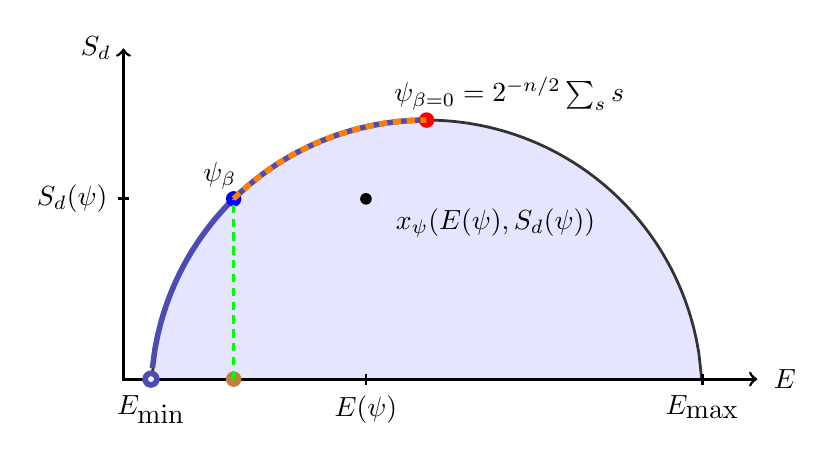
\begin{tikzpicture}[scale=3.5,
declare function={
        func(\x) = sqrt(\x*(2-\x))-0.06;
      }]

\begin{scope}
\clip (-0.1,1.2) rectangle (2.2,0);
\draw[black!80!white, line width=1pt, domain=0:2,fill=blue!10!white, samples=200]  plot (\x,{func(\x)});
\end{scope}
\draw[gray!60!blue, line width=2pt, domain=0.005:1, samples=100]  plot (\x,{func(\x)});

\draw [<->, line width=1pt] (-0.1,1.2) -- (-0.1,0) -- (2.2,0);
\node[] at (-0.2,1.2) { $S_d$};
\node[] at (2.3,0) { $E$};
 
% free and bound energy
\fill (1.,{func(1)}) circle (.6pt);
\node[above] at (1.3,{func(1)}) { $\ket{\psi_{\beta=0}}=2^{-n/2}\sum_s\ket{s}$};
\fill (.3,{func(.3)}) circle (.6pt);
\node[above] at (.25,{func(.3)}) {$\ket{\psi_\beta}$};
\fill (.78,{func(.3)}) circle (.6pt);
\node[below] at (1.25,{func(.3)}) {$x_\psi\coloneqq(E(\psi),S_d(\psi))$};
\draw [line width=1pt] (0.78,.02) -- (.78,-.02) node[below] {$E(\psi)$};
\draw [line width=1pt] (2,.02) -- (2,-.02) node[below] {$E_{\textrm{max}}$};
\draw [line width=1pt] (0.0,.02) -- (0,-.02) node[below] {$E_{\textrm{min}}$};
\fill [color=gray!60!blue](0,0) circle (.9pt);
\fill [color=white](0,0) circle (.3pt);

\fill [color=blue](0.3,{func(.3)}) circle (0.8pt);
\fill [color=red](1,{func(1)}) circle (0.8pt);
\fill [color=brown](0.3,0) circle (.8pt);

\draw [green, densely dashed, line width=1pt] (0.3,0) -- (0.3,{func(.3)});

\draw[orange, densely dashed, line width=2pt, domain=0.3:1, samples=100]  plot (\x,{func(\x)});

\draw [line width=1pt] (-0.08,{func(.3)}) -- (-.12,{func(.3)}) node[left] {$S_d(\psi)$};
\end{tikzpicture}

\caption{estados de interés en el diagrama entropía-energía}
\label{fig:energy-entropy-diagram-mod}
\end{center}
\end{figure*}

De esta forma comparamos los estados de Gibbs a una temperatura dada, energía y entropía fija, con los estados que comparten características similares pero no exactamente iguales.

\newpage

Los estados situados a lo largo de la linea verde, incluido el punto marrón, poseen la misma energía que el estado de Gibbs, representado por el punto azul, pero menor entropía. Por otro lado, los estados de Gibbs, situados a los largo de la linea naranja incluido el punto rojo, poseen mayor entropía que el estado de Gibbs pero también mayor energía. Para comparar la calidad de la solución obtenida por el algoritmo QAOA inicializado con el estado correspondiente, se usará la diferencia de energía relativa denotada por $\alpha$. La diferencia de energía relativa viene dado por la expresión \ref{eq:diference_relative}. Un valor positivo de $\alpha_{r}(x,y)$ implicaría que la calidad de la solución de $y$ es mayor que la de $x$, dado que la calidad de energía relativa $\alpha$ es máxima cuando toma el valor cero.

\begin{equation}
    \alpha_{r}(x, y) = \alpha(x) - \alpha(y) = \frac{|E_{exacta}| - |E_{x}|}{|E_{exacta}|} - \frac{|E_{exacta}| - |E_{y}|}{|E_{exacta}|}
    \label{eq:diference_relative}
\end{equation}

En primer lugar, presentamos el gráfico dado por la Figura \ref{fig:gibbs_product}, la cual compara estados de Gibbs, punto azul, con estados producto, punto marrón.

\begin{figure}[!h]
    \centering
    \includegraphics[scale = 0.7]{plt/06-gibbs_vs_producto.png}
    \caption{diferencia relativa de energía entre estados de Gibbs y estados producto a $T=4$}
    \label{fig:gibbs_product}
\end{figure}

En la Figura \ref{fig:gibbs_product} se muestra como varía $\alpha_{r}$(estado producto, estado Gibbs) con el tamaño del problema. \\ 

Se puede observar que de forma consistente, independientemente del tamaño del problema o del numero de capas del algoritmo QAOA, la calidad de la solución obtenida por el algoritmo es mejor cuando este se inicializa con estados de Gibbs en lugar de estados producto que poseen la misma energía de partida. Cada diagrama de caja del gráfico es el resultado de 30 simulaciones, lo que da un total de 540 simulaciones llevadas a cabo para la generación del gráfico (ver apéndice \ref{apendix:product_vs_hadamard} para más detalle). \\

La siguiente gráfica presentada, dada por la Figura \ref{fig:gibbs_hadamard_nodes} compara estados de Gibbs,  punto azul, con el estado Hadamard, punto rojo, a una temperatura fija de $T=4$, es decir se presenta $\alpha_{r}$(estado Hadamard, estado Gibbs). 

\begin{figure}[!h]
    \centering
    \includegraphics[scale = 0.7]{plt/06-gibbs_vs_hadamard_nodes.png}
    \caption{diferencia relativa de energía entre estados de Gibbs y el estado Hadamard a $T=4$}
    \label{fig:gibbs_hadamard_nodes}
\end{figure}

Al igual que con la Figura \ref{fig:gibbs_product}, el algoritmo QAOA, inicializado con estados de Gibbs a temperatura $T=4$, arroja un rendimiento superior, independientemente del numero de capas. 

\newpage

Se puede observar como un aumento del tamaño del problema genera una mayor distancia entre la calidad de la solución obtenida por el QAOA inicializado con el estado Hadamard y el QAOA inicializado por el estado de Gibbs. Este hecho se produce debido a que la energía de partida del estado Hadamard es creciente con el tamaño del problema, dado que es un promedio energético de todas las soluciones posibles del problema. De igual forma, cada diagrama de caja ha sido el resultado de 30 simulaciones, lo que da un total de 420 simulaciones llevadas a cabo para la generación del gráfico. \\


La siguiente gráfica que se presenta, es también una comparación entre estados de Gibbs y estados Hadamard, pero ahora a un tamaño de problema fijo, en el cual se varia la temperatura. Lo que se va a comparar es como varia $\alpha_{r}$(estado Hadamard, estado Gibbs) cuando nos desplazamos a lo largo de la linea naranja del diagrama \ref{fig:energy-entropy-diagram-mod}. En la Figura \ref{fig:gibbs_hadamard_temperature} se presenta dicha comparación para un problema de tamaño $N=16$.

\begin{figure}[!h]
    \centering
    \includegraphics[scale = 0.75]{plt/06-gibbs_vs_hadamard_temperature.png}
    \caption{diferencia relativa de energía entre estados de Gibbs y el estado Hadamard con $N=16$}
    \label{fig:gibbs_hadamard_temperature}
\end{figure}

\newpage

Se puede observar en la Figura \ref{fig:gibbs_hadamard_temperature} como a medida que nos desplazamos a lo largo de la linea naranja, lo cual es equivalente a estados de Gibbs de menor temperatura, tal como marca la relación \ref{eq:time_temperature}, la diferencia de calidad entre el estado Hadamard y el estado de Gibbs especifico aumenta. Además podemos observar que la función es monótona creciente dado que una reducción en la temperatura implica necesariamente una mejora en la calidad de la solución obtenida por el QAOA.  De igual forma, cada diagrama de caja ha sido el resultado de 30 simulaciones, lo que da un total de 420 simulaciones llevadas a cabo para la generación del gráfico. \\

Las Figuras \ref{fig:gibbs_hadamard_nodes} y \ref{fig:gibbs_hadamard_temperature} son además de especial utilidad para mostrar la potencia de los estados de Gibbs puros. En numerosos artículos del estado de la técnica, como el trabajo de \cite{shaydulin}, muestran numéricamente que para el algoritmo QAOA, los estados que maximizan el rendimiento del algoritmo son los estados fundamentales del Hamiltoniano de mezcla, que para el caso del QAOA genérico, es el estado Hadamard. No obstante aquí se comprueba que existen otros estados no triviales, que consiguen un rendimiento del QAOA consistentemente mejor que el estado Hadamard. \\

Por último, queda comparar los estados de Gibbs con aquellos estados que poseen una misma energía pero distinta entropía no nula, es decir aquellos estados situados a lo largo de la linea verde del diagrama \ref{fig:energy-entropy-diagram-mod}. Tal y como se puede observar en la gráfica \ref{fig:entropia_vs_energia_pseudogibbs}, dado un conjunto de estados donde todos ellos poseen la misma energía, pero distinta entropía, aquellos que maximizan el rendimiento del algoritmo QAOA son aquellos que poseen entropía de coherencia máxima. La normalización de la entropía asociada a cada estado se realiza en base a la entropía del estado de Gibbs en ese punto, dado que a una energía determinada, dicho estado maximiza la entropía. Es claro, que a medida que nos acercamos al limite del Boltzmann, es decir, aumentamos la entropía del estado de inicialización, la calidad de la solución arrojada por el algoritmo QAOA, en forma de energía relativa con respecto a la solución exacta, aumenta de forma consistente. \\

La metodología llevada a cabo para la construcción de estados de \textit{pseudoGibbs}, es decir estados cercanos al limite del Boltzmann, ha sido mediante la creación de estados gaussianos. Dado un estado de Gibbs a temperatura $T$, dicho estado posee una energía fija $E_{T}$.


\newpage

\begin{figure}[!h]
    \centering
    \includegraphics[scale = 0.75]{plt/06-entropia_vs_energia_pesudo_gibbs.png}
    \caption{calidad de la solución obtenida en función de la entropía del estado de pseudoGibbs para tamaños de $N=9$}
    \label{fig:entropia_vs_energia_pseudogibbs}
\end{figure}

Para construir estados gaussianos que representan estados de pseudoGibbs utilizamos la expresión dada por \ref{eq:psgibbs_state}.

\begin{equation}
    \ket{\psi_{\text{psGibbs}}(E_{T})} = \frac{1}{\sigma \sqrt{2 \pi}} \sum_{i}e^{-\frac{(E_{i} - E_{T})^2}{2 \sigma^2}} \ket{i}
    \label{eq:psgibbs_state}
\end{equation}

Donde $\ket{i}$ son los estados propios del Hamiltoniano, $E_{i}$ es el valor propio de la energía asociado al estado $\ket{i}$, $E_T$ es el valor en el cual se centra la gaussiana y donde $\sigma$ es la desviación estandar de la gaussiana, es decir la anchura de la distribución normal. Mediante el parámetro $\sigma$ podemos controlar la cantidad de estados que participan en la combinación lineal del estado de pseudoGibbs que posee energía $E_T$, es decir que podemos controlar la entropía del estado. Un valor de $\sigma$ mas alto, implica una mayor cantidad de estados que participan de la combinación lineal, aumentando así la entropía. \\

A traves de esta metodología, hemos podido validar numéricamente la hipotesis presentada en el apartado \ref{sub_sec:hip_work} para el caso del algoritmo variacional QAOA. Una forma alternativa de visualizar los resultados presentados que es mas intuitiva y descriptiva, aunque solo es el resultado de un caso particular, aunque aleatorio, es mediante un mapa de calor. 

\newpage

Usando el diagrama de entropía-energía podemos representar la calidad de los resultados obtenidos por el algoritmo QAOA en función de estados de inicialización y ordenarlos según el propio diagrama entropía-energía. En la Figura \ref{fig:mapa_calor} puede observarse el mapa de calor de un problema concreto de Max Cut de 10 nodos para un QAOA de 3 capas.


\begin{figure}[!h]
    \centering
    \includegraphics[scale = 0.8]{plt/06-mapa_calor.png}
    \caption{mapa de calor del algoritmo QAOA de tres capas para un problema de $N=8$}
    \label{fig:mapa_calor}
\end{figure}

Se puede observar que según el mapa de calor presentado, los estados que maximizan el rendimiento del algoritmo QAOA, aquellos estados que de inicialización que maximizan la calidad de la solución obtenida por QAOA, son los estados del limite de Boltzmann. Por otro lado, los estados situados en el núcleo del diagrama son aquellos que peor rendimiento arrojan como estados de inicialización (ver apéndice \ref{apendix:energy_landscape}  para más detalle). Para evitar que aquellos estados que ya se encuentran cerca del mínimo arrojen soluciones mejores solo por el hecho de encontrarse cerca del estado exacto, la energía final del QAOA presentada como código de colores dentro de la Figura \ref{fig:mapa_calor}, se normaliza con respecto a la energía final del QAOA obtenida por los estados de Gibbs en cada punto.

\newpage

De esta forma, la calidad de la solución se compara siempre con respecto a los estados de Gibbs, y tal como puede observarse, no hay ningún estado dentro del diagrama que mejore la solución obtenida por los estados de Gibbs.

\section{Protocolos de pre-optimización}

Habiendo mostrado evidencias numéricas de que los estados de Gibbs puros, situados en el limite de Boltzmann maximizan el rendimiento del algoritmo QAOA, podemos aseverar que el protocolo mostrado en la sección \ref{sub_sec:dmrg} arrojará un rendimiento peor que el protocolo novedoso presentado en la sección \ref{sub_sec:i_tevo}. No obstante es difícil comparar justamente ambos protocolos dado que son bastante diferente entre ellos. El algoritmo de tensor networks de pre-optimización es totalmente distinto, usando el primer protocolo el algoritmo DMRG y el segundo, el algoritmo MPO Time Evolution. Además, los \mbox{PQC} utilizados también difieren, ya que el primero utiliza un conjunto de puertas cuánticas de dos qubits $SU(4)$ con una cantidad de parámetros a optimizar, creciente con el tamaño del problema, mientras que el segundo utiliza un \mbox{PQC} fijo para la preparación del estado de inicialización con un conjunto de capas de QAOA añadidas para ser optimizadas. \\

No obstante podemos presentar un conjunto de gráficas, que muestran el rendimiento dispar que poseen ambos protocolos de pre-optimización cuando se pretende resolver un problema clásico como el Max Cut. En la Figura \ref{fig:comparativa_protocolo} comparamos ambos métodos de pre-optimización para resolver un problema concreto de Max Cut de un grafo de $N=10$. Se puede observar que, aunque el algoritmo DMRG del primer protocolo converge mas rápido a un estado de menor energía posteriormente, el algoritmo VQE es incapaz de  mejorar el resultado de partida dado por el algoritmo DMRG. El motivo de esto, se debe a que el algoritmo DMRG a convergido a un estado de baja energía pero también de baja entropía. En terminos del diagrama \ref{fig:energy-entropy-diagram}, el algoritmo DMRG a convergido a un estado que se encuentra muy alejado del limite de Boltzmann. Así pues, el algoritmo VQE empieza en un mínimo local del que no puede escapar y por tanto no puede mejorar el resultado de partida. Por otro lado, el algoritmo MPO Time Evolution es más lento en converger a estados de menor energía, ya que para igual número de pasos de optimización o tiempo de evolución, según sea el algoritmo de tensor networks, el algoritmo MPO Time Evolution arroja estados de mayor energía que los encontrados por el DMRG. 

\newpage

\begin{figure}[!h]
    \centering
    \includegraphics[scale = 0.7]{plt/06-comparativa_protocolo.png}
    \caption{comparativa de rendimiento de los protocolos de pre-optimización}
    \label{fig:comparativa_protocolo}
\end{figure}


No obstante, dado que el estado final construido por el algoritmo MPO Time Evolution es un estado de Gibbs puro de temperatura $T$, el algoritmo QAOA inicializado con dicho estado, consigue mejorar el punto de partida y mejorar al mismo tiempo el resultado conseguido por el protocolo DMRG-VQE. Además por los resultados presentados en el apartado \ref{sub_sec:result_gibbs_states}, se puede aseverar que bajo el estado de inicialización de Gibbs el algoritmo QAOA maximiza su rendimiento. \\

Otra comparativa que se podría realizar es comparar el rendimiento del algoritmo QAOA con ambos algoritmos de pre-optimización para asegurar que la diferencia de rendimiento no solo se debe por un cambio del PQC utilizado. No obstante, esta es una prueba redundante, ya que las gráficas presentadas en el apartado \ref{sub_sec:result_gibbs_states} muestran que los estados de Gibbs maximizan el rendimiento contra cualquier otro estado que esté lejos del limite de Boltzmann. El estado solución que genera el algoritmo DMRG es un estado que solo trata de minimizar $\braket{H}$ sin atender al grado de entropía del estado, por lo tanto, de forma usual el algoritmo DMRG arrojará estados solución que se encuentren alejados del limite de Boltzmann.

\newpage

Una última que es importante realizar es la diferencia de rendimiento del algoritmo VQA, en este caso el algoritmo QAOA con y sin el uso del protocolo de pre-optimización, es decir, comparar la ventaja que se obtiene cuando se utiliza un QAOA que no ha utilizado la pre-optimización con otro que si se ha servido de ello. En la Figura \ref{fig:itevo_qaoa} se compara cual es el rendimiento del algoritmo QAOA cuando trata de resolver un problema especifico de Max Cut de $N=6$ con un QAOA de $p=8$ capas.


\begin{figure}[!h]
    \centering
    \includegraphics[scale = 0.7]{plt/06-itevo_qaoa.png}
    \caption{comparativa de rendimiento entre QAOA e ITEVO-QAOA}
    \label{fig:itevo_qaoa}
\end{figure}

Tal y como puede verse en la Figura \ref{fig:itevo_qaoa}, cuando el QAOA se inicializa con un estado inicial Hadamard, un estado de Gibbs de temperatura infinita, el algoritmo QAOA parte de un estado enérgicamente alto y se queda atrapado en mínimos locales que son sub-óptimos. Sin embargo, si se inicializa el algoritmo QAOA con estados de Gibbs de menor temperatura, el algoritmo QAOA parte de posiciones enérgicamente más favorables, lo que le da mayor capacidad de encontrar el mínimo global. Las líneas discontinuas de la Figura \ref{fig:itevo_qaoa} hacen referencia a la energía final del estado generado por el algoritmo MPO Time Evolution para cada una de las temperaturas correspondientes.

\newpage

\section{Código desarrollado}

Como parte de la colaboración \textbf{UNIR-Qilimanjaro} para el desarrollo y realización del trabajo presentado, se ha hecho uso de paquetes propios de Qilimanjaro. Esto impide la publicación en su totalidad del código en repositorios de acceso publico. No obstante, parte sustancial del código, el cual permite replicar toda la sección \ref{sub_sec:result_gibbs_states} se encuentra en la siguiente dirección \url{https://github.com/anavasca/TFM-Gibbs-States.git}. Además, en dicho repositorio se encuentran los datos en brutos obtenidos de las simulaciones numéricas. Estos datos han sido los utilizados para generar todas las figuras presentadas en el capítulo de \textit{discusión de resultados}. El resto del código utilizado queda disponible, si así se desea, bajo solicitud previa para ser validado. Para la solicitud del código contactar con \href{mailto:anavascaliz@gmail.com}{anavascaliz@gmail.com}. \\

El código cuántico se ha desarrollado en el lenguaje Qibo. Este lenguaje es análogo a otros como Qiskit, Pennylane o Circ. Por otro lado, para el desarrollo de los algoritmos de tensor networks implementados, se ha hecho uso de la librería numpy de Python. Además, todas las simulaciones llevadas a cabo han sido realizadas en ordenadores clásicos mediante simulaciones. No se ha probado nada de lo mostrado en ordenadores cuánticos reales, dado el coste en terminos de tiempo que se requiere. Es por ello que todas las ejecuciones y resultados mostrados han sido llevados a cabo en servidores clásicos. En particular, se ha utilizado un servidor propiedad de Qilimanjaro denominado como \textit{Radagast}, el cual posee 60 Gb de memoria RAM y 18 nodos de cálculo. Gracias a disponer de los recursos clásicos mencionados, se han podido llevar a cabo un gran numero de simulaciones. 